\def\mytitle{Optimization Assignment}
\def\myauthor{Hari Venkateswarlu Annam}
\def\contact{hariannam99@gmail.com}
\def\mymodule{Future Wireless Communication (FWC)}
\documentclass[10pt, a4paper]{article}
\usepackage[a4paper,outer=1.5cm,inner=1.5cm,top=1.75cm,bottom=1.5cm]{geometry}
\twocolumn
\usepackage{graphicx}
\graphicspath{{./images/}}
\usepackage[colorlinks,linkcolor={black},citecolor={blue!80!black},urlcolor={blue!80!black}]{hyperref}
\usepackage[parfill]{parskip}
\usepackage{lmodern}
\usepackage{tikz}
\usepackage{physics}
\usepackage{tabularx}
\usetikzlibrary{calc}
\usepackage{amsmath}
\usepackage{amssymb}
\renewcommand*\familydefault{\sfdefault}
\usepackage{watermark}
\usepackage{lipsum}
\usepackage{xcolor}
\usepackage{listings}
\usepackage{float}
\usepackage{titlesec}
\providecommand{\mtx}[1]{\mathbf{#1}}
\titlespacing{\subsection}{1pt}{\parskip}{3pt}
\titlespacing{\subsubsection}{0pt}{\parskip}{-\parskip}
\titlespacing{\paragraph}{0pt}{\parskip}{\parskip}
\newcommand{\figuremacro}[5]{
    \begin{figure}[#1]
        \centering
        \includegraphics[width=#5\columnwidth]{#2}
        \caption[#3]{\textbf{#3}#4}
        \label{fig:#2}
    \end{figure}
}
\newcommand{\myvec}[1]{\ensuremath{\begin{pmatrix}#1\end{pmatrix}}}
\let\vec\mathbf
\lstset{
frame=single, 
breaklines=true,
columns=fullflexible
}
\thiswatermark{\centering \put(0,-105.0){
\includegraphics[scale=0.08]{iith_logo}} }
\title{\mytitle}
\author{\myauthor\hspace{1em}\\\contact\\IITH\hspace{0.5em}-\hspace{0.5em}\mymodule}
\date{}
\begin{document}
	\maketitle
\paragraph{\textit{Problem Statement}}- Show that the shortest distance from a given point to a given straight line is the perpendicular distance.

\section*{\large Solution}
\begin{figure}[H]
\centering
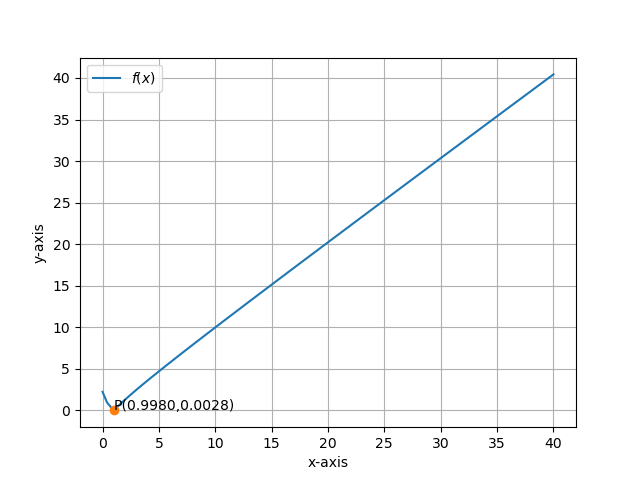
\includegraphics[width=1\columnwidth]{Figure1.png}
\caption{Graph}
\label{fig:triangle}
\end{figure}
\textbf{Assumptions :}
Let us assume (2,2) be the given point and x+y=2 be the given line,\\
line and point in vector form \\

\begin{align}
\vec{P} = \myvec{2\\2}\\
\vec{n}^T\vec{x}=c\\
\vec{x}=\vec{A}+\lambda \vec{m}\\
\vec{A} = \myvec{2\\0}, \vec{m} = \myvec{1\\-1}\\
d^2 = \norm{\vec{P}-\vec{x}}^2\\
d^2 = \norm{\vec{P}-(\vec{A}+\lambda \vec{m})}^2
\end{align}
\begin{align}
	\label{eq:one}
	d^2 = \lambda^2\norm{\vec{m}}^2-\lambda(2(\vec{P}-\vec{A})^T\vec{m})+\norm{\vec{P}-\vec{A}}^2
	\end{align}
by substituting P,A,m in \eqref{eq:one}
\begin{align}
	\label{eq:two}
	d^2 = \lambda^2\norm{\myvec{1\\-1}}^2-2\lambda\left[\left (\myvec{2\\2}-\myvec{2\\0}\right)^T\myvec{1\\-1}\right]
+\norm{\myvec{2\\2}-\myvec{2\\0}}^2
	\end{align}
	by solving \eqref{eq:two} we get,
\begin{align}
d^2=2(\lambda^2+2\lambda+2)
\end{align}
\textbf{Obective Function :}
\begin{align}
d^2=2(\lambda^2+2\lambda+2)
\end{align}

    \subsection*{\normalsize Gradient descent method}
    
    \begin{align}
	\label{eq:vol_varx}
	f(x) = 2(x^2+2x+2)
\end{align}
\begin{align}   
    f'(x) = 2(2x+2)
	\end{align}
we have to attain the maximum value of m. This can be seen in Figure.Using gradient descent method we can find its minima value.
\begin{equation}
        x_{n+1} = x_n - \alpha \nabla f(x_n) \\
\end{equation}
\vspace{1mm}
\begin{equation}
\implies x_{n+1}=x_n+\alpha2(2x+2)
\end{equation}
Taking $x_0=0.5,\alpha=0.001$ and precision = 0.00000001, values obtained using python are:
    \begin{align}
        \text{Minima} = 1.414\\        
        \text{Minima Point} = -1\\
        \implies \lambda=-1\\
         d_p=\frac{|n^T\vec{P}-c|}{\norm{\vec{n}}+++}\\
         d_p = 1.414 
    \end{align}
Hence,the shortest distance from a given point to a given straight line is perpendicular distance.    
   \end{document}
